\documentclass[letterpaper,12pt]{article}
% Soporte para los acentos.
\usepackage[utf8]{inputenc}
\usepackage[T1]{fontenc}
% Idioma español.
\usepackage[spanish,mexico, es-tabla]{babel}
% Soporte de símbolos adicionales (matemáticas)
\usepackage{multirow}
\usepackage{amsmath}
\usepackage{amssymb}
\usepackage{amsthm}
\usepackage{amsfonts}
\usepackage{latexsym}
\usepackage{enumerate}
\usepackage{ragged2e}
\usepackage{mathtools}

% Soporte para referencias y citas
\usepackage{hyperref}

% Soporte para imágenes.
\usepackage{graphicx}
% Modificamos los márgenes del documento.
\usepackage[lmargin=2cm,rmargin=2cm,top=2cm,bottom=2cm]{geometry}


    \title{Fundamentos de Bases de Datos \\
        Tarea 1 \\
        Conceptos básicos}


    \author{Teresa Becerril Torres
            $\#$ de cuenta: $315045132$ \\
            Miguel Ángel Torres Sánchez
            $\#$ de cuenta: $315300442$ \\
            Nicole Romina Traschikoff García
            $\#$ de cuenta: $315164482$ \\
            Tania Michelle Rubí Rojas
            $\#$ de cuenta: $315121719$}
        \date{18 de febrero del 2019}

    \begin{document}
    \maketitle

    \section{Conceptos generales.}
          \begin{enumerate}[a. ]

            \item ¿Por qué elegirías almacenar datos en un \textbf{sistema de base de datos} en lugar de simplemente almacenarlos utilizando el \textbf{sistema de archivos} de un sistema operativo? ¿En qué casos no tendría sentido utilizar un sistema de base de datos? \\

          Porque en una base de datos bien diseñada se asegura la integridad de los datos y facilita trabajar con ellos a usuarios y desarrolladores. No tendría sentido usar una base de datos cuando los usuarios son pocos y cuando las cantidades de información no son grandes y no crecerán mucho o no existirá por largos periodos de tiempo.

            \item ¿Qué \textbf{ventajas} y \textbf{desventajas} encuentras al trabajar con una \textbf{base de datos}?\\

            Las ventajas que proporciona trabajar con una base de datos son aquellas garantías que nos da su diseño y el sistema manejador de bases de datos, es decir, brinda chequeo de redundancia, operaciones básicas, integridad de datos y la posibilidad de seguir expandiendo un sistema robusto, además de poder recuperar la información de manera práctica y eficiente.

            Por otro lado las desventajas principales pueden estar relacionadas a los alcances del propio diseño de la BDs, donde el modelo no permita representar las necesidades de la organización, instalación costosa, se necesita de personal especializado, etc.


            \item Investiga cuáles serían las \textbf{responsabilidades} de una \textbf{DBA} y las de un \textbf{diseñador de bases de datos.}
            
            \begin{enumerate}
              \item Las responsabilidades de un \textbf{DBA} son:
              \begin{itemize}
                  \item Autorizar el acceso a la base de datos. 
                  \item Coordinar y monitorear el uso de la base de datos.
                  \item Adquirir recursos de software y hardware según sea necesario.
                  \item Asegurar la confiabilidad de la base de datos.
                  \item Proteger la seguridad de la base de datos.
              \end{itemize}
  
              \item Las responsabilidades de un \textbf{diseñador de bases de datos son}:
              \begin{itemize}
                  \item Identificar los datos que se almacenarán en la base de datos.
                  \item Elegir las estructuras apropiadas para representar y almacenar los datos.
                  \item Crear un diseño que cumpla con los requisitos de todos los posibles usuarios de la base de datos
              \end{itemize}  
      \end{enumerate}
            \item Investiga cuáles serían los distintos tipos de usuarios finales de una base de datos, indica las principales \\

          Las categorías de ususarios finales de una base de datos son:

        	\begin{itemize}
        		\item Usuario casual: acceden ocasionalmente a la base de datos con la necesidad de información diversa.
        		\item Usuario paramétrico: consultan y actualizan constantemente la base de datos con funciones ya programadas y probadas.
        		\item Usuario sofisticado: conocen bien el SMBD para implementar aplicaciones que cumplan requisitos complejos.
        		\item Usuario independiente: utiliza paquetes de software específicos fáciles de usar para mantener una base de datos personal.
        	\end{itemize}

            \item Explica las diferencias entre la \textbf{independencia de datos física} y \textbf{lógica}. ¿Cuál es más difícil de lograr y por qué?

            \textsc{Solución:} La independencia de datos física es cuando los cambios en la organización física de la base de datos no afectan al mundo exterior (es decir, los programas o los usuarios directos), mientras que la independencia de datos lógica es cuando los usuarios no se ven afectados por los cambios a nivel lógico (ya sean cambios en el esquema conceptual o cambios en los esquemas externos). La independencia lógica es más difícil de lograr ya que los programas de aplicación son muy independientes de la estructura lógica de los datos a los que accede (se han creado a partir de ella).

            \item ¿Qué es un \textbf{diccionario de datos} y por qué es importante para el SMBD? \\
            
            Un \textbf{diccionario de datos} es un conjunto de definiciones de otros objetos del sistema. Es importante para el SMBD ya que proporciona información acerca de:
            \begin{itemize}
              \item Estructura lógica y física de la base de datos.
              \item Definición de todos los objetos de la base de datos. 
              \item Espacio asignado y utilizado por los objetos.
              \item Valores por omisión en las columnas.
              \item Información acerca de las restricciones de integridad.
              \item Privilegios y roles otorgados a los usuarios.
              \item Estadísticas de utilización, frecuencias de consultas, de transacciones y el número de accesos a diferentes porciones de la base de datos.
            \end{itemize}

            \item Indica las principales características de los modelos de datos más representativos. ¿Cuáles serían las
            diferencias entre los modelos relacional, orientado a objetos, semiestructurado y objeto-relacional? \\
          \begin{itemize}

            \item \textbf{Modelo relacional}. Es basado en tablas. Todo el procesamiento se realiza sobre tablas y el resultado son tablas.
            \item \textbf{Modelo orientado a objetos}. Los datos se modelan como objetos con estado y comportamiento.

            \item \textbf{Modelo semiestructurado}. Representación de los datos menos rígida. Colección de nodos con su propia descripción de los datos.

            \item \textbf{Modelo objeto-relacional}. Aprovecha características de datos en tablas y objetos.

          \end{itemize}

          La diferencia entre los modelos está en cómo representan los datos, los modelos relacional y orientado a objetos tienen una estructura rígida mientras que el modelo semiestructurado es el más flexible.\\

            \item Elabora una \textbf{línea de tiempo}, en dónde indiques \textbf{los principales hitos} en el desarrollo de las BDs.\\\\
          {\Large\itshape \textbf{Principales hitos en el desarrollo de las Bases de Datos} \par}
          \vspace{.5cm}
          \vfill


                  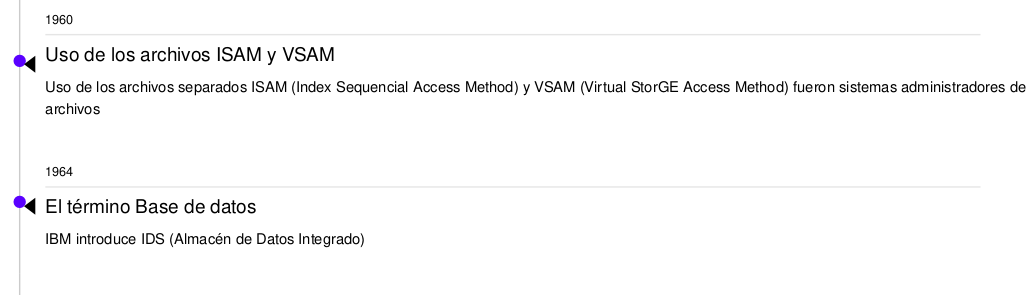
\includegraphics[width=\textwidth]{imagenes/parte1.png}
                  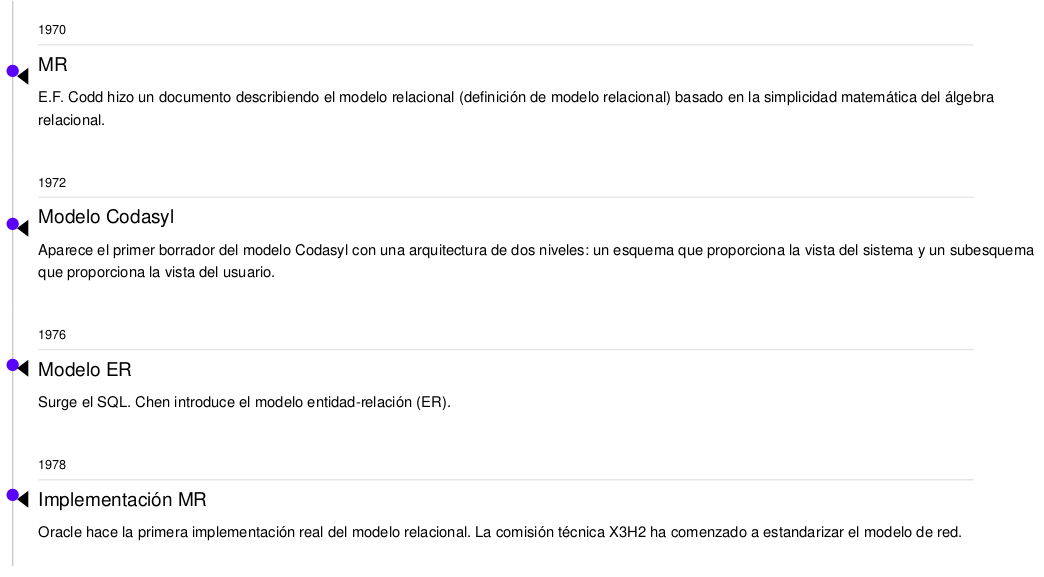
\includegraphics[width=\textwidth]{imagenes/parte2.png}
                  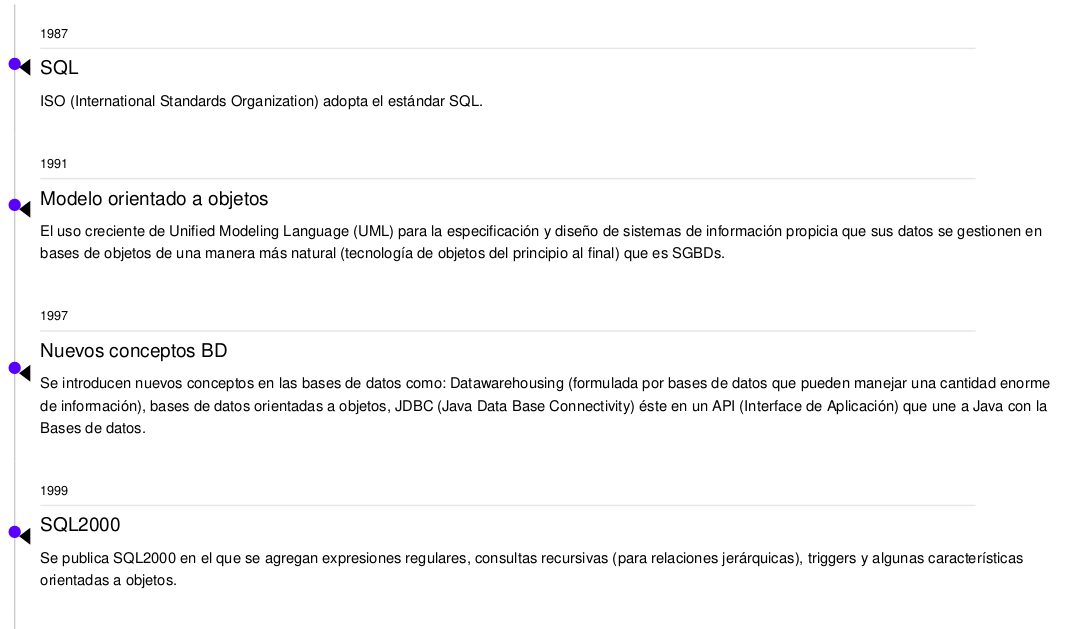
\includegraphics[width=\textwidth]{imagenes/parte3.png}
                  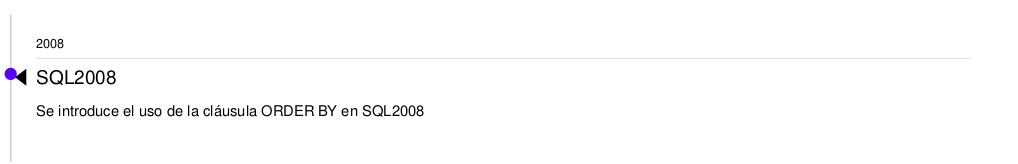
\includegraphics[width=\textwidth]{imagenes/parte4.png}


            \item Indica las responsabilidades que tiene un \textbf{Sistema Manejador de Bases de Datos} y para cada responsabilidad, explica los problemas que surgirían sí dicha responsabilidad no se cumpliera. \\


            \item Supón que un banco pequeño desea almacenarlos su información en una base de datos y le gustaría comprar el SMBD que tenga la menor cantidad de características posibles. Está interesado en ejecutar la aplicación en una sola computadora personal y no se planea compartir la información con nadie. Para cada una de las siguientescaracterísticas explica por qué se debería o no incluir en el SMBD que desea comprar (suponiendo que se pueden comprar por separado:) \textbf{seguridad, control de concurrencia, recuperación en caso de fallas, lenguaje de consulta, mecanismo de vistas, manejo de transacciones.} \\
          \end{enumerate}

            \section{Investigación.}
            \begin{enumerate}[a)]

            \item ¿Qué es la \textbf{Calidad de Datos} y cómo se relaciona con las bases de datos? \\
        	Calidad de datos se refiere a las técnicas y procesos utilizados para asegurar que un dato es adecuado para su uso en operaciones y toma de decisiones. Se relaciona con las bases de datos pues debido a la gran cantidad de información que tienen se debe asegurar que todos los datos sirven su propósito ya que de no hacerlo podría tenerse información incorrecta o poner en riesgo la seguridad de la base de datos.

            \item ¿Qué son las bases de datos \textbf{NoSQL}? indica el modelo de datos utilizado y algunos proveedores.\\

         Los sistemas de bases de datos relacionales llevan décadas siendo el modelo informático más empleado del mundo para almacenar y recuperar la información.\\

         Pero este sistema ha ido cambiando en los últimos años, surgió una contracorriente con el propósito de defender las bases de datos que no utilizaban el lenguaje SQL, denominado como el movimiento \textbf{\textit{ NoSQL}}. \\

         Las bases de datos \textit{NoSQL} son un modelo no relacional, los defensores de las bases de datos NoSQL argumentan que pueden evitar la complejidad innecesaria, proporcionan en general, un alto rendimiento, pueden manejar una gran cantidad de datos, soportar lenguajes de consulta de tipo SQL y hardware de bajo costo, entre otros.\\

          Y estos son algunos de sus proveedores.
          \begin{itemize}
            \item Hypertable
            \item Cassandra
            \item MongoDB
            \item DynamoDB
            \item HBase
            \item Redis

          \end{itemize}




            \item ¿Qué es un \textbf{Almacén de datos}? Indica las diferencias entre éstos y una base de datos.

            \end{enumerate}


            \section*{Referencias}
            \begin{itemize}

            	\item Elmasri, R. and Navathe, S. B. \textbf{Fundamentals of Database Systems}. Addison-Wesley Publishing Company, Sexta edición, 2011.
            	\item Redman, T. C. \textbf{Data Driven: Profiting from Your Most important Business Asset}. Harvard Business Press, 2008.

              \item Anodrea Rodríguez M.\textbf{Introducción a Bases de Datos}. Universidad de Concepción, Chile. 2007.

              \item URL: \url{http://www.ptolomeo.unam.mx:8080/xmlui/bitstream/handle/132.248.52.100/219/A6.pdf?sequence=6}

              \item



            \end{itemize}

            \end{document}
